%!TEX root = ../thesis.tex
\chapter{Features to be Personalised} % (fold)
\label{ch:analysis}
This section analyses the user preferences and identifies which features should be modelled as personalisation constraints. It also seeks to define the default setting that consists the general model for a good editorial mix of a digital newspaper.

The focus of automatically generating the editorial mix introduces temporal, spacial and relational circumstances about the composition. But before these can be modelled as constraints it is necessary to look at the user needs of the application.
%
 %These will consist the content constraints of the system along with those determined by user preferences. Therefore the constraints that belongs to composition conditions must be presented/defined.

Some prerequisites must be stated in order to set the focus of the problem, but also for the potential user to relate to the product. The research done by \cite{FULLTEXT01.pdf} and \cite{kristin_fredrik.pdf} determines the preferable size of the digital newspaper to be $14.732 \times 20.828$cm $\sim$ size A5, which reflects the size of the iPad. Therefore this project will target the iPad as its primary device. The handheld device also introduces mobility, which is also of great preference to the potential users.
%
%\begin{itemize}
	%\item $14.732 \times 20.828$cm $\sim$ size A5, which reflects the size of the iPad% \cite[p. 1]{FULLTEXT01.pdf} % \cite[p. 6-7]{kristin_fredrik.pdf}
	%\item reader knows about constraints
	%\item relevance feedback introduced (click on article, time spend reading it and scroll)
	%\item argument that transparency of the general model is enough for the user to provide settings \cite[p. 7]{gervasum2001ws.pdf}
%\end{itemize}

\section{User Needs}
This section will define the user needs for the application. A full description of personas, scenarios and business case is found in appendix~\vref{appendix:user-needs}.

After the definition of the initial requirements was done the first prototype was developed. Its main features followed the requirements on turning pages, choosing an article, read it and returning to the overview of articles, see Figure~\ref{fig:prototype-iteration1}.

\begin{figure}%
%\centering%
\makebox[\textwidth][r]{% %%% as above; this time, the
%%% figures flushes from the left
\subfloat[Initial prototype layout with adjustable ratios between articles and a paged interface of each section.\label{fig:prototype-iteration1}]%
	{\includegraphics[width=.38\largefigure]{img/prototype-iteration1}}%
	\qquad%
\subfloat[Second iteration of the prototype with an ``endless'' layout. Sections are placed beneath each other.\label{fig:prototype-iteration2}]%
	{\includegraphics[width=.38\largefigure]{img/prototype-iteration2}}%
}
\\
\makebox[\textwidth][r]{% %%% as above; this time, the
\subfloat[Third iteration of the prototype with a column-based and ``endless'' layout. Sections are placed beneath each other.\label{fig:prototype-iteration3-1}]%
	{\includegraphics[width=.38\largefigure]{img/prototype-iteration3-1}}%
	\qquad%
\subfloat[Third iteration of the prototype with a column-based and ``endless'' layout. Sections are placed beneath each other.\label{fig:prototype-iteration3-2}]%
	{\includegraphics[width=.38\largefigure]{img/prototype-iteration3-2}}%
}
\caption{The figure shows three iterations of the prototype layout.}%
\label{fig:prototype-iterations}%
\end{figure}

After a preliminary small survey it became clear, that a column-based layout would be more attractive, and would provide a better opportunity to explore the editorial mix. With a column-based layout the digital newspaper would have more resemblance to conventional newspapers and therefore it was possible to apply some of the same principles of the editorial mix.

After the second prototype was developed it was tested. A specification of the test can be found in Table~\ref{tab:test-description}.

\begin{table}[h!tp]
	\caption{Test Specification}
	\label{tab:test-description}
	\myfloatalign
		\begin{tabularx}{\textwidth}{p{.2\textwidth}|p{.7\textwidth}}
		\toprule
			\textbf{Test subjects} & The test was conducted on a total of 7 test subjects of ages between 21-29, and of different sex and occupation.\\
		\midrule
			\textbf{Participants} & Each test was done with 1 test conductor and 1 test subject.\\
		\midrule
			\textbf{Materials} & An iPad with the application running and a computer to write notes on the test subject's statements and propositions.\\
		\midrule
			\textbf{Description} & The test subject was presented with the prototype layout seen in Figure~\ref{fig:prototype-iteration3-1} and~\ref{fig:prototype-iteration3-2}. The test was conducted as an informal qualitative talk with a basis in the test subject's interests in such a product. Transcripts from each test can be found at \url{lestrade.imm.dtu.dk/~ArtistRecommender/data/test-transcripts.zip}.\\
		\bottomrule
		\end{tabularx}
\end{table}

The prototype consisted of the basic navigation between subject categories, i.e.\ sections, and articles. Navigational choices was made in order to present the general idea of the framework, but where more crucial choices on its uses have not been made jet. This was also to encourage the test subjects to talk about what uses they would have of the presented framework. However, they were also asked about the navigational structure and indeed some changes had to be done.

The above presented preparatory work resulted in the following user needs:
\begin{itemize}
	\item Read articles presented in a nice and digestible layout
	\item Get an easy overview of the content of the newspaper
	\item Easily navigate between articles with few touch-friendly interactions
	\item Read relevant articles based on user defined subjects
\end{itemize}

\section{Use Cases}
These user needs and the results from the conducted tests proposes some use cases from the application. Theses will presented here.

In order to fulfil the user needs more general use cases are derived. These and the web servers handling of them are shown in Figure~\ref{fig:use-cases}.

%\sidecaptionfigure{\textwidth}{img/use-cases}{The figure shows the overall use cases of the system and how the web server acts to accomplish them.}{fig:use-cases}
\begin{figure}[h!tp]
	\centering
	
	\def\mygraphic{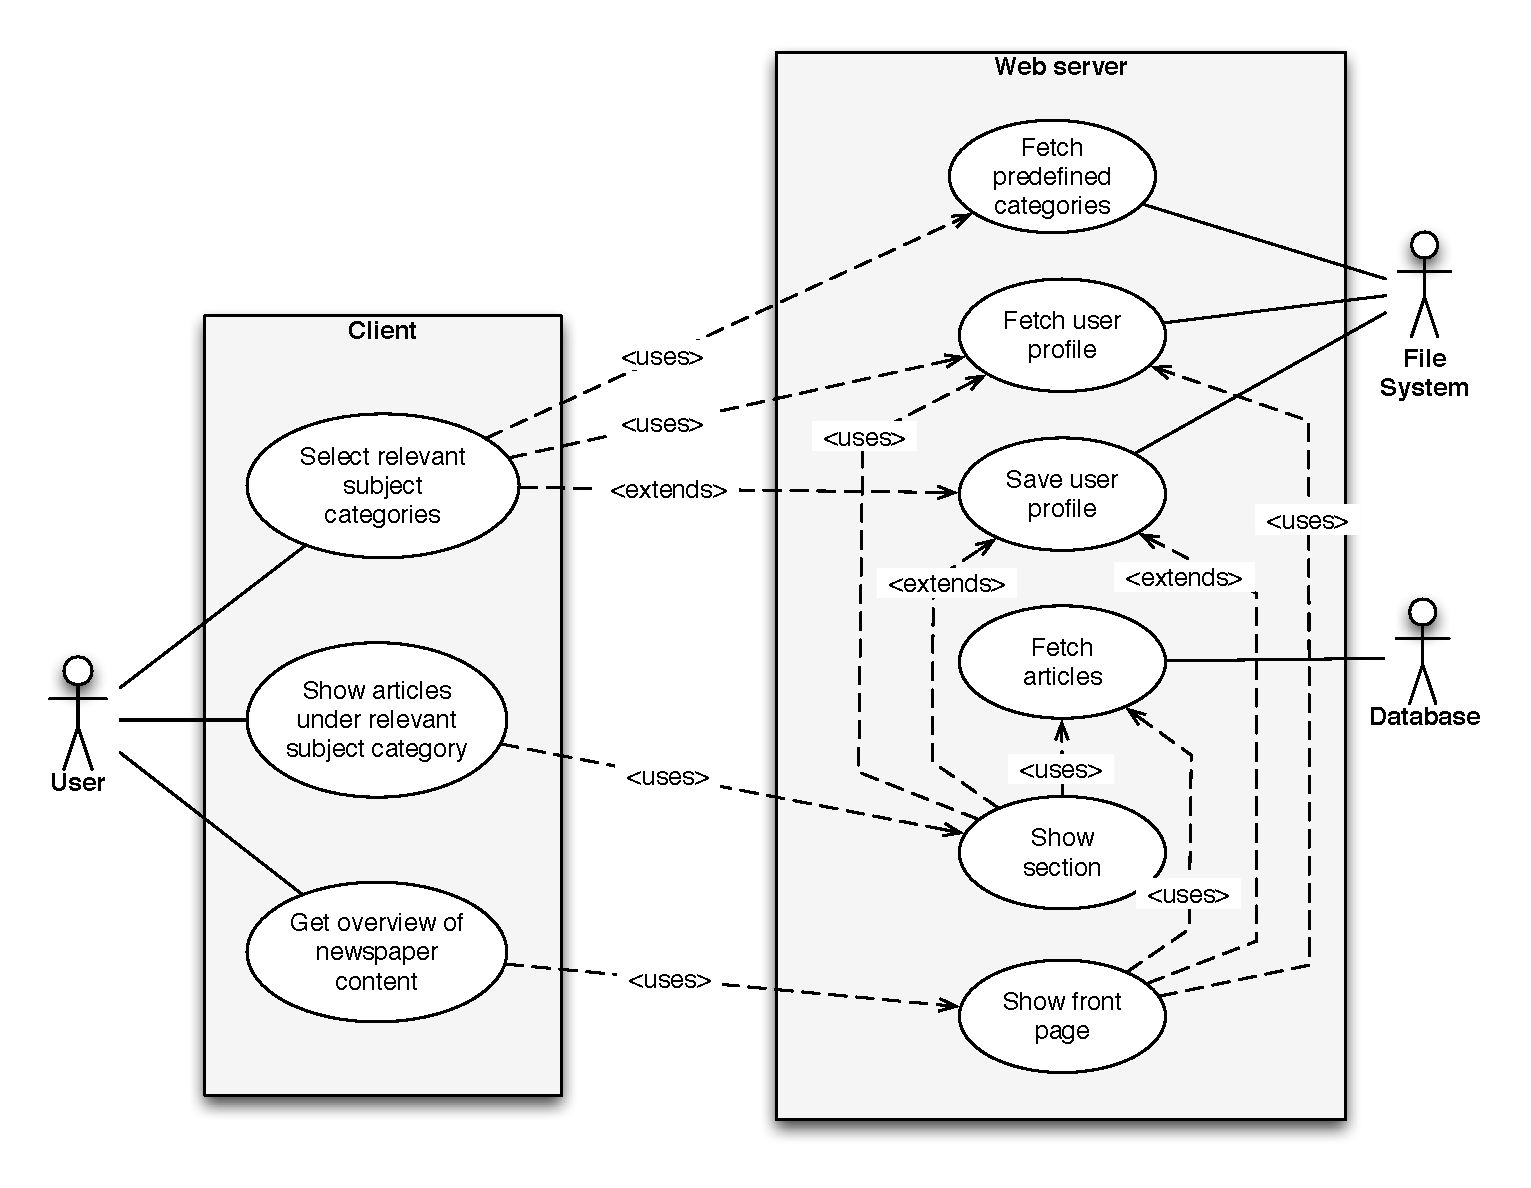
\includegraphics[width=\textwidth]{img/use-cases}}
	%\newlength{\graphicheight}
	\settoheight\graphicheight{\mygraphic}
	\mygraphic
	\marginnote{
	\begin{minipage}{\marginparwidth}
		\vspace{-\graphicheight}%
		\caption{The figure shows the overall use cases of the system and how the web server acts to accomplish them.}
		\label{fig:use-cases}
		\vspace{\graphicheight}
		\end{minipage}
	}
\end{figure}

The list of use cases shown in the figure are by no means a complete, but are selected because they have the closest relation to the user needs.

The user is able to select relevant subject categories to get an easy start with the application and the choices are thereafter saved to the user profile for later use. The user can select a subject category from the earlier chosen categories and browse articles from this subject within a section. If the user needs to get an overview of the content of the newspaper he can get the front page displayed, which contains a small collection of articles of most interest to the user.

In Figure~\ref{fig:sequence} is shown a sequence diagram of what the system does in order to display the front page (or a section), when the user opens the application.
%\sidecaptionfigure{\textwidth}{img/sequence}{The figure shows a sequence diagram from when the user chooses a subject category until he can read articles from this subject. \texttt{secNum} is the section number to display (the front page is section 0), \texttt{userId} is a string that identifies the user, \texttt{userPrefs} is the user preferences on the specific section and \texttt{articles} is the library of articles to compose the editorial mix of.}{fig:sequence}
\begin{figure}[h!tp]
	\centering
	
	\def\mygraphic{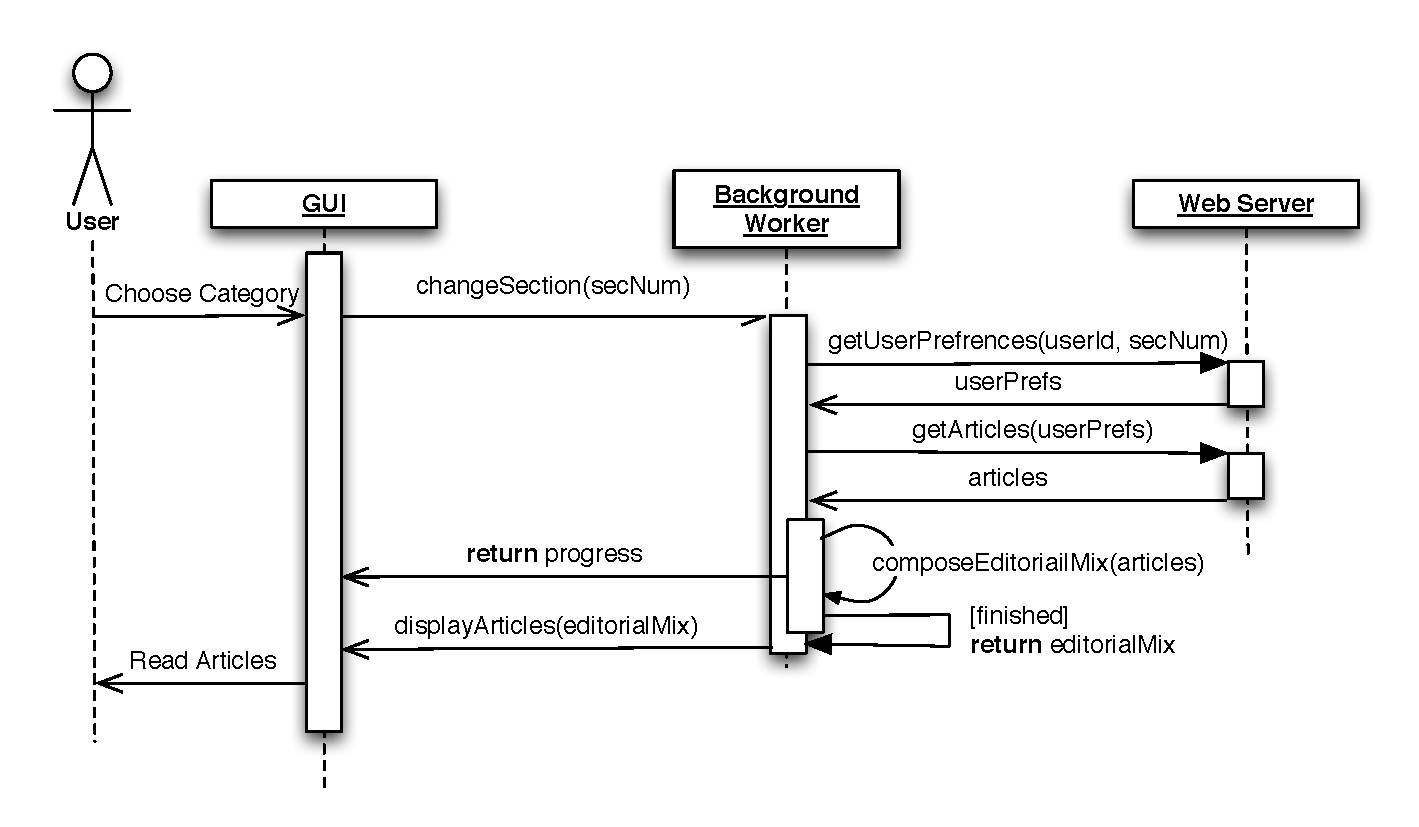
\includegraphics[width=\textwidth]{img/sequence}}
	\settoheight\graphicheight{\mygraphic}
	\mygraphic
	\marginnote{
	\begin{minipage}{\marginparwidth}
		\vspace{-\graphicheight}%
		\caption{The figure shows a sequence diagram from when the user chooses a subject category until he can read articles from this subject. \texttt{secNum} is the section number to display (the front page is section 0), \texttt{userId} is a string that identifies the user, \texttt{userPrefs} is the user preferences on the specific section and \texttt{articles} is the library of articles to compose the editorial mix of.}
		\label{fig:sequence}
		\vspace{\graphicheight}
		\end{minipage}
	}
\end{figure}
%\begin{figure}[h!tp]
%	\myfloatalign
%		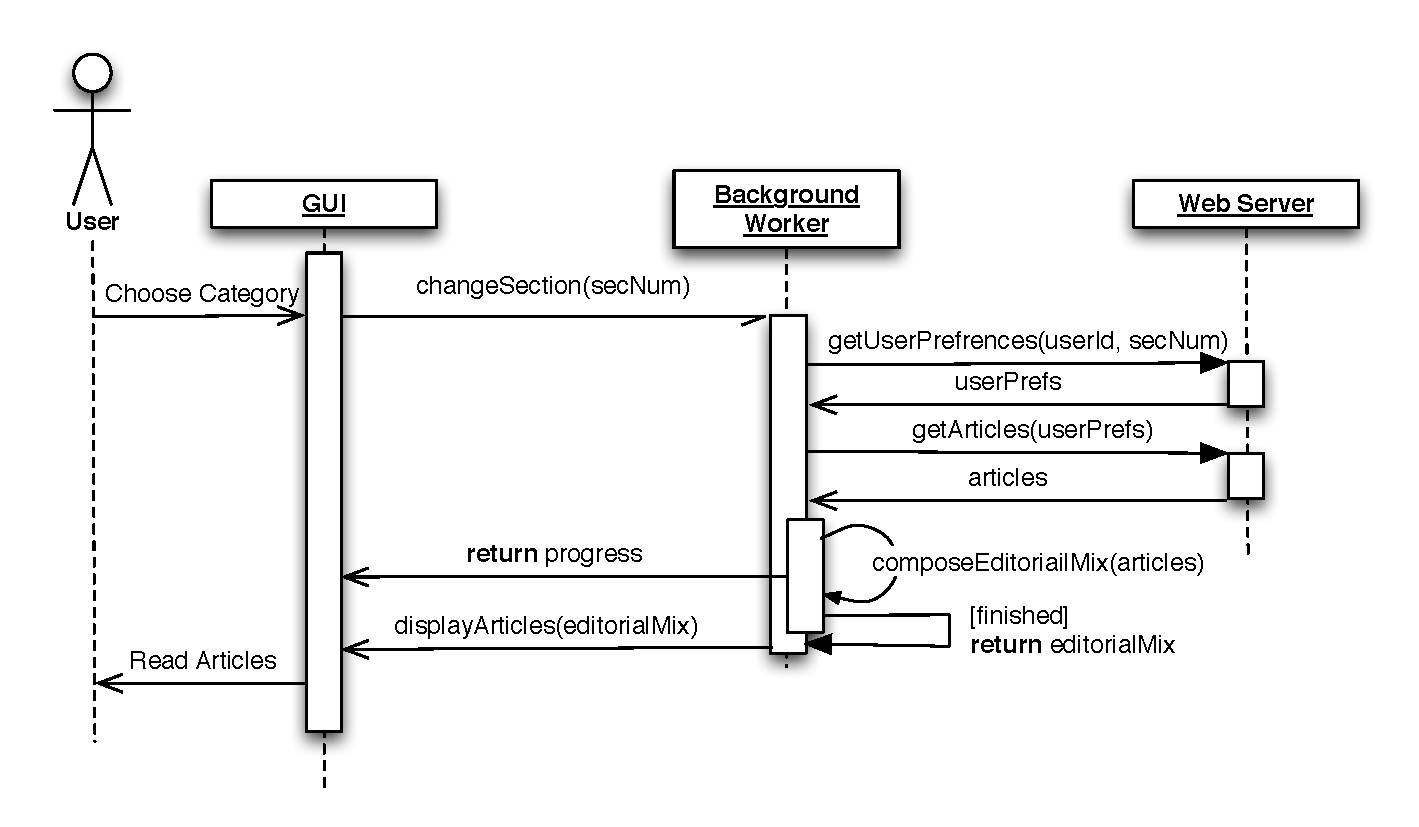
\includegraphics[width=\textwidth]{img/sequence}
%	\caption{The figure shows a sequence diagram from when the user chooses a subject category until he can read articles from this subject. \texttt{secNum} is the section number to display (the front page is section 0), \texttt{userId} is a string that identifies the user, \texttt{userPrefs} is the user preferences on the specific section and \texttt{articles} is the library of articles to compose the editorial mix of.}
%	\label{fig:sequence}
%\end{figure}

When the application is opened, or the application is changed to display a section, a background worker is initialised to compose its containing mix of articles. Of cause, if the mix of articles in a section, or front page, have already been computed, it does not need to recompute it. The background worker needs to get both the user preferences of the chosen category and article that potentially fit the user preferences. While worker computes the editorial mix it sends messages to the user interface about the progress. When it finishes the user interface is asked to display the articles.

\section{Requirements}
\subsection{Non-functional Requirements}
In the explored literature and the conducted tests users express some non-functional requirements. These are described in this section.

User needs states the requirement of having a clear overview of the content and as stated in \cite{FULLTEXT01.pdf}, this includes a clear marking of the beginning and the end of the articles and sections. This is obtained by both having a summery of the most interesting articles on the front page and by having a dropdown list of headlines in the top of section.

From the user needs it is also required that the system should be easily navigated and as stated by \cite{kristin_fredrik.pdf}, this should be through clickable sections, headlines and through paging. The layout, typography and design should be familiar to what is found in conventional newspapers, as stated by \cite{FULLTEXT01.pdf} and \cite{hcii2005_1004.pdf}. This is achieved by choosing a structure that resembles that of a newspaper and displaying content in balanced columns. It should be possible for the user to read the newspaper screen by screen, meaning that trailing text should be put into a new set of columns whenever it exceeds the screen, see Figure~\ref{fig:reading2} and \ref{fig:reading1}.

%\begin{figure}[h!tp]
%\myfloatalign
%\subfloat[Reading pattern where the user has to scroll in order to see the full length of the column.]{
%  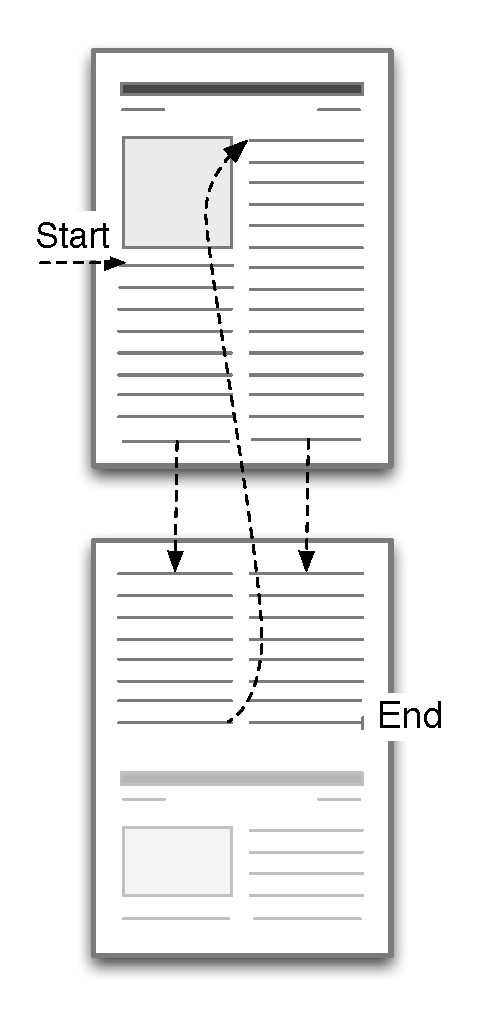
\includegraphics[width=.3\textwidth]{img/reading1}
%  \label{fig:reading1}
%} \qquad
%\subfloat[Reading pattern where the user can finish reading a whole page before scrolling to read the next.]{
%  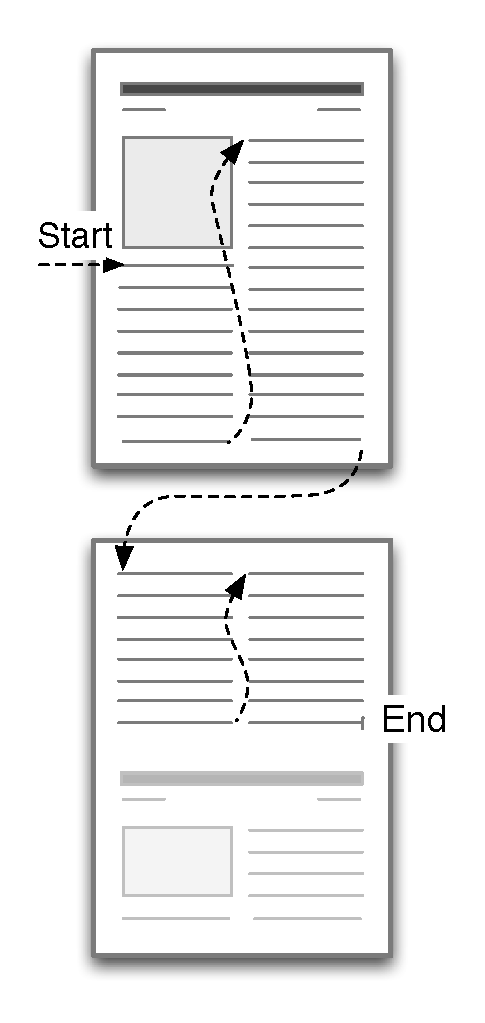
\includegraphics[width=.3\textwidth]{img/reading2}
%  \label{fig:reading2}
%}
%\caption{The figure shows two examples of reading patterns in a column based layout.}
%\label{fig:reading}
%\end{figure}

\begin{sidefigure}%
\centering%
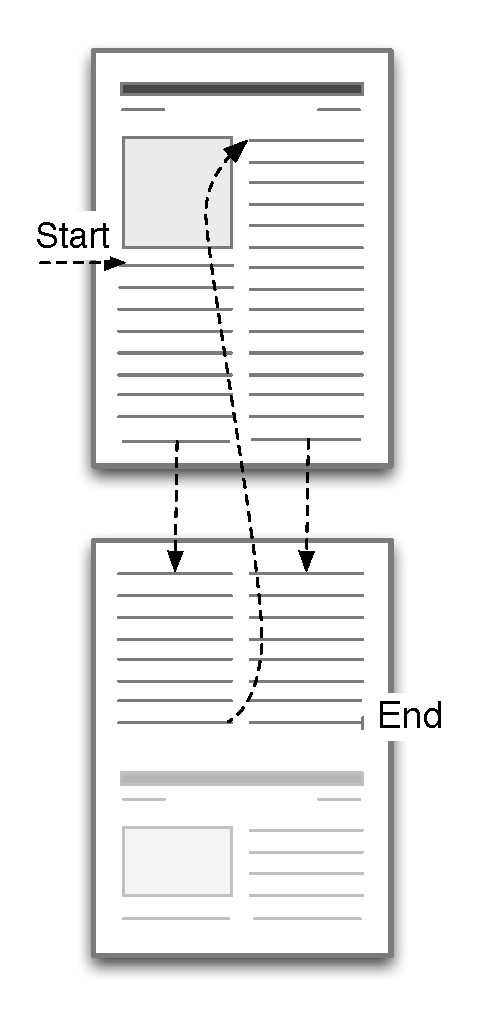
\includegraphics[width=\marginparwidth]{img/reading1} 
\caption{Reading pattern where the user has to scroll in order to see the full length of the column.}%
\label{fig:reading1}%
\end{sidefigure}

\begin{sidefigure}%
\centering%
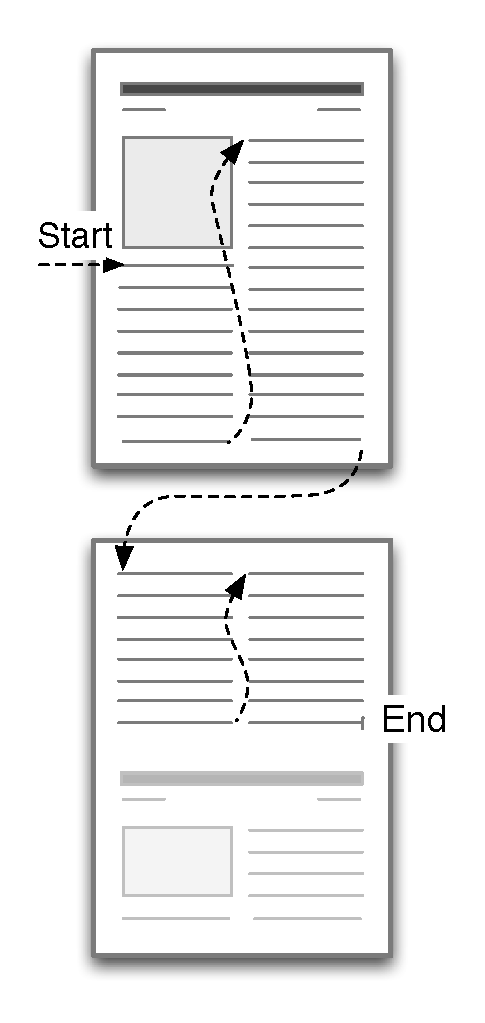
\includegraphics[width=\marginparwidth]{img/reading2} 
\caption{Reading pattern where the user can finish reading a whole page before scrolling to read the next.}%
\label{fig:reading2}%
\end{sidefigure}

\begin{itemize}
	\item Ease of use
	\item both general and personal news (collaborate filtering solves that some news are not received, but are universally interesting \cite{fulltext.pdf})
	
	\item both images and videos - test
	\item a good ratio of graphical and textual - test
	
	\item front page should give a good overview of the content - test
	\item ``news valuation, e.g. positioning of lead story'' \cite[p. 7]{FULLTEXT01.pdf}
	\item  mobility \cite[p. 7]{FULLTEXT01.pdf}
	\item  continuous updates \cite[p. 7]{FULLTEXT01.pdf}
	\item ``easy and intuitive navigation'' \cite[p. 7]{FULLTEXT01.pdf}
	\item add video and sound \cite[p. 7]{FULLTEXT01.pdf}
	\item incorporate social community and social networks
\end{itemize}

\subsection{Functional Requirements}
Some technical requirements have also been gathered from the explored literature.
\begin{itemize}
	\item ``open, turn pages, chose article, read and return'' \cite[p. 6]{FULLTEXT01.pdf}
	\item section headlines \cite[p. 6-7]{kristin_fredrik.pdf}
	\item article headlines
	\item article summaries / extracts \cite{fulltext.pdf}
	\item menu w. section headlines \cite[p. 8]{kristin_fredrik.pdf}
	\item page numbers \cite[p. 6-7]{kristin_fredrik.pdf}
	\item press ``like'' or key word based user profile (mark self or highlighted? right click to add): positive + negative list (keywords+categories \cite{10-1-1-19-5583}, \cite{fulltext.pdf} and \cite{gervasum2001ws.pdf})
	\item full screen display of article
	\item organise into personalised sections
	\item opens in front page view (summery of newspaper 8 articles) \cite[p. 8]{kristin_fredrik.pdf}
	\item adjust variables
	\item share directly (grey out the ones who have read it)
	\item comment
	\item see friends comments
	\item ``The presentation schema -- headline, abstract, and text, together with a relevance value with respect to the user profile -- rates the highest in terms of user satisfaction, and yet it is not the most frequent.'' \cite{Sections-categories-and-keywords-as-interest-specification-tools-for-personalised-news-services.pdf}
	\item  ability to search \cite[p. 7]{FULLTEXT01.pdf}
	\item Landscape + portrait \cite[p. 6-7]{kristin_fredrik.pdf}
	\item touch screen interaction \cite[p. 6-7]{kristin_fredrik.pdf}
	\item Functionality from online newspaper \cite{hcii2005_1004.pdf}
	\item Name of columnist \cite[p. 4]{gervasum2001ws.pdf}
	\item Transparency of implicit relevance feedback (see/modify current weights of categories) \cite[p. 7]{gervasum2001ws.pdf}
	\item dynamic short-term + static long-term user profile \cite{10-1-1-19-5583}, \cite{fulltext.pdf} and \cite{gervasum2001ws.pdf}
	\item relevance feedback \cite{10-1-1-19-5583}, \cite{fulltext.pdf} and \cite{gervasum2001ws.pdf}
\end{itemize}

%
%\subsection{Non-functional Requirements}
%\begin{itemize}
%	\item a good ratio between general and personal news
%	\item a good ratio between graphical and textual content
%	\item incorporation social network and community
%	\item a good reading flow
%\end{itemize}
%
%\subsection{Functional Requirements}
%Some technical requirements have also been gathered from the explored literature.
%\begin{itemize}
%	
%	\item easy navigation
%	\item contemplated typography and design
%	\item most interesting articles on the front page
%	\item opens in front page view (summery of newspaper few articles)
%	\item navigation through section headlines, article headlines and article summaries / excerpts
%	\item back page, funnies?
%	\item put in personalised sections
%	\item relevance value by article
%	\item menu with section headlines
%	\item page numbers
%	\item page turn
%	\item possibility of relevance feedback
%	\item keyword based user profile
%	\item ability to adjust preference variables
%	\item full screen display of article
%	\item columns should be divided to fit into one screen with possible images or videos
%	\item familiarity in design and layout from printed paper
%	\item news valuation, e.g.\ positioning of lead story
%	\item continuous updates
%	\item ability to search
%	\item video and sound
%	\item should be readable in both landscape and portrait
%	\item touch screen interaction
%	\item Functionality from online newspaper
%	\item Name of columnist
%	\item Transparency of implicit relevance feedback (see/modify current weights of categories)
%	\item dynamic short-term + static long-term user profile
%	\item relevance feedback
%\end{itemize}
%
\section{Delimitation}
The proposed design in chapter~\vref{ch:design} should of cause account for requirements, but there are some requirements that will not be implemented due to prioritisation and time limits

The initial approach involved computing the tf-idf similarity between documents and the user and the documents in between using the Python libraries for this \cite{NLTK}. This approach works on a bow (bag-of-words) with key words and weights representing a single item. The weight is computed by the number of occurrences in the provided text and a cosine distance determines the similarity. Python also provides an interface for working with WordNet -- a large lexical database of English words and their relationships in the form of different graphs. This opens the door to a more in-depth analysis of the optained news items. \cite{116262780379.pdf} presents an algorithm for enriching articles using WordNet's hypernym-graphs. A hypernym graph is generated by the top $20\%$ frequent keywords of an article and weighted by:
$$W(d, f) = 2 \cdot \frac{1}{1+e^{-0.125(d^3\frac{f}{TW})}}-0.5$$

Where $d$ stands for the node's depth in the graph (starting from root and moving downwards), $f$ is the frequency of appearance of the node to the multiple graph paths and $TW$ is the total number of words used to generate the hypernym graph.

In order to be able to work with hypernyms, the words must be converted to synsets. For each word there exists a synset for each use of the word, with the most frequently used first. Every synset is included at this point, but in a later stage this could be further focused by only using the top $n$. An analysis on how many percent of the words

\todo[inline]{Which design choices to focus on?}
Introduce columns and remove pages to introduce newspaper like layout

Do not focus on summaries -- out of scope, 

Support images only, not video -- can easily be introduced.

Not implement support for social networking, but included in the proposed design

Predefined categories is not a full list, but are of the most recurring in popular news sites.

\todo[inline]{In which period of time is an article relevant to a user? Maybe if it is still available, then it is still interesting -- new approaches or discussion about the subject might arise. How do we control that a news item is not missed? Keep index of what has been viewed in addition to what has been read.}


% section analysis (end)
